We designed and implemented a Jupyter kernel for MMT.
We describe its interface in Section~\ref{sec:kernel:syntax} and the implementation in Section~\ref{sec:kernel:impl}.

\subsection{Interface}\label{sec:kernel:syntax}

MMT differs from typical computational engines in Jupyter in that it does not only (and not even primarily) perform computation but also handles symbolic expressions with uninterpreted function symbols, whose semantics is described by logical axioms.
Another important difference is how MMT handles context and background knowledge.
Kernels for (mathematics-oriented or general purpose) programming languages, as typical in Jupyter, build and maintain a dynamic context of declarations with imperative assignment and stack-oriented shadowing and rely on a fixed --- often object-oriented --- background library of computational functionality.
MMT, on the other hand, uses graphs of inter-connected theories to represent a multitude of possible contexts and background libraries and to move knowledge between contexts.
To adequately handle these subtleties, we systematically specified a new interface for Jupyter-style interactions with MMT.

\paragraph{Sessions}
Jupyter interactions are managed in \textbf{sessions}: every browser page opening a notebook creates a new session.
Sessions are represented as MMT documents, which gives them a unique URI.
All commands executed within a session manipulate the associated document, most importantly by interactively creating new theories and then calling MMT algorithms on them.
The latter include but are not limited to computation.

\paragraph{Input}
The possible inputs excepted by the MMT kernel are divided into three groups.
\begin{itemize}
\item \textbf{Global management commands} allow displaying and deleting all current sessions.
 In practice, these commands are typically not available to common users, which should only have access to their own session.
\item \textbf{Local management commands} allow starting, quitting, and restarting the current session. These are the main commands issued by the frontend in response to user action.
\item \textbf{Content commands} are the mathematically meaningful commands and described below.
\end{itemize}

The content commands are divided into two groups:
\begin{itemize}
 \item \textbf{Write-commands} send new content to the backend in order to build the current MMT document step by step.
   The backend maintains one implicit, ephemeral MMT document for each session, and any write command changes that document.
 \item \textbf{Read-commands} retrieve information from the backend without changing the session's document.
   These include lookups (both in the session document and in any other accessible document) or computations.
\end{itemize}

A write-command typically consists of a single MMT declaration roughly corresponding to a line in a typical MMT source file.
However, the nesting of declarations is very important in MMT.
This is in contrast to many programming language kernels where nesting is often optional, e.g., to define new functions or classes;
for many current kernels, it makes sense to simplify the implementation by requiring that the entire top-level command, including any nesting, be contained in a single cell.

In our MMT kernel, all declarations that may contain nested declarations (most importantly all MMT documents and theories) are split into parts as follows: the header, the list of nested declarations, and a special end-of-nesting marker.
Each of these is communicated in a separate write-command.
The semantics of MMT is carefully designed in such a way that (i) any local scope arising from nesting has a unique URI, and (ii) if a well-formed MMT document is built incrementally by appending individual declarations to a currently open local scope, any intermediate document is also well-formed.
This is critical to make our implementation feasible: the MMT kernel maintains the current document as well as the URI of the current scope; any write-command affects the current scope, possibly closing it or creating new subscopes.
This ensures that all nested declarations are parsed and interpreted in the right scope.

For example, the sequence of commands on the left of Figure~\ref{fig:test_theory} builds two nested theories, where the inner one refers to the type \texttt{a} declared in the outer one.
The right-hand side of Figure~\ref{fig:test_theory} shows the equivalent MMT surface syntax on the right.
Semantically, there is no difference between entering the left-hand side interactively via our new kernel or processing the right-hand side with the old MMT parser.
\begin{figure}[ht]\centering
\begin{minipage}[c]{10cm}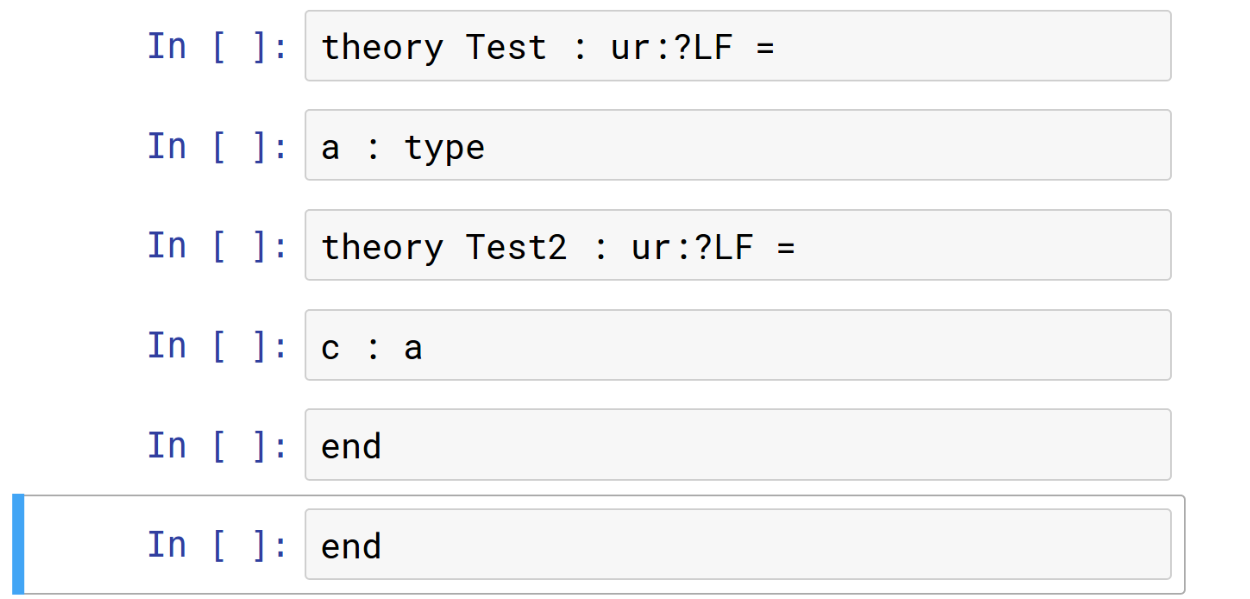
\includegraphics[width=10cm]{test_theory_jupyter}\end{minipage}
\begin{minipage}[c]{5cm}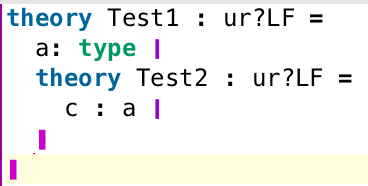
\includegraphics[width=5cm]{test_theory}\end{minipage}
\caption{Content Commands for Building Theory Graphs}\label{fig:test_theory}
\end{figure}

A special write-command is \texttt{eval T}.
It interprets \texttt{T} in the current scope, infers its type \texttt{A}, computes its value \texttt{V}, and then adds the declaration \texttt{resI:A=V} to the current theory, where \texttt{I} is a running counter of unnamed declarations.
This corresponds most closely to the REPL functionality in typical Jupyter kernels.

While write-commands correspond closely to the available types of MMT declarations, the set of read-commands is extensible.
For example, the commands \texttt{get U} where \texttt{U} is any MMT URI returns the MMT declaration of that URI.

\paragraph{Output}
The kernel returns the following kinds of return messages:
\begin{itemize}
\item \textbf{Admin messages} are strings returned in response to session management commands.
\item \textbf{New-element messages} return the declaration that was added by a write-command.
\item \textbf{Existing-element messages} return the declaration that was retrieved by a \texttt{get} command.
\end{itemize}
Like read-commands, the set of output messages is extensible.

The new-element and existing-element messages initially return the declaration in MMT's abstract syntax.
And a post-processing layer specific to Jupyter renders them in HTML+presentation MathML.
That way, the core kernel functionality can be reused easily in other frontends than Jupyter.

\subsection{Implementation}\label{sec:kernel:impl}

\paragraph{Overview}
Generally, Jupyter emphasizes protocols that specify the communication between frontend (i.e., usually Jupyter notebooks) and backend (i.e., kernels implemented in various programming languages).
This requires a certain duplication of implementation and, critically, maintenance, e.g., when implementing xeus, xwidgets and similar libraries for C++.
But the Python infrastructure for kernels is by far the best developed one, especially when it comes to Jupyter widgets. 
Therefore, it makes sense to implement our kernel on top of Python.
However, actually executing the user's commands requires a strong integration with the MMT implementation, which uses Scala.
That made it advisable to implement all Jupyter-specific functionality, especially the communication and management, in Python, while all mathematically relevant logic is handled in Scala.

Therefore, our implementation consists of three layers.
The top layer is a Python module that implements the abstract class for Jupyter kernels.
The bottom layer is a Scala class adding a general-purpose REPL to MMT that handles all the logic of MMT documents.
This can be reused easily in other frontends.
User commands are entered on the client and sent to the top layer, which forwards all requests to the bottom layer and all responses from the bottom layer to the client.
The communication between top and bottom layer is handled by a middle layer.
Its main purpose is to bridge between Python and MMT, format results in HTML, and add interactive functionality via widgets.

This bridging of programming languages is a generally difficult problem.
After some experiments with different solutions (e.g., HTTP communication) and discussion within the OpenDreamKit community, we identified the Py4J library~\cite{Py4J:on} as the best choice.
This is a Python-JVM bridge that allows seamless interaction between Python and any language (such as Scala) that compiles to the JVM.
Thus, our Python kernel can call MMT code directly.
Valuable Py4j features include callbacks from MMT to Python, shared memory (by treating pointers to JVM objects as Python values), and synchronized garbage collection.
That makes our kernel very robust against bit rot and allows benefiting from future improvements to the MMT backend.

Py4J is only JVM-specific, not Scala-specific.
That means that some Scala-specific constructs are not readily exposed to Python.
For example, both Python and Scala allow magic methods for treating any object as a function, but the JVM does not; moreover, the magic method is called \texttt{\_\_call\_\_} in Python and \texttt{apply} in Scala.
Similarly, Scala collections like lists are not automatically seen as their counterparts in Python.
Therefore, we wrote a Python module (which is distributed with MMT\footnote{This is currently at \url{https://github.com/UniFormal/MMT/blob/devel/src/python-mmt/example/mmt.py} but may be moved in the future.}) that performs the bureaucracy of matching up advanced Python and Scala features.


\subsection{Graphical User Interfaces via Jupyter Widgets}

Jupyter widgets are interactive GUI components (e.g., input fields, sliders, etc.) that allow Jupyter kernels to provide graphical interfaces.
While the concept is general, it is most commonly used to refer to the Python-based widget library developed for the Python kernel.
A widget encapsulates state that is maintained in an instance of a Python class on the server and displayed via a corresponding Javascript/HTML component on the client.
A major advantage of our kernel design is that we can reuse these widgets (via the to layer).

As our kernel's intelligence is maintained is maintained in MMT and thus Scala, we had to write some middle layer code to allow our kernel to create widgets.
This code uses Py4J to expose the widget-management functionality of the top layer to the lower layers.
This is done via a class of callback functions $C$ that are passed along when the former calls the latter.

\begin{figure}[ht]\centering
  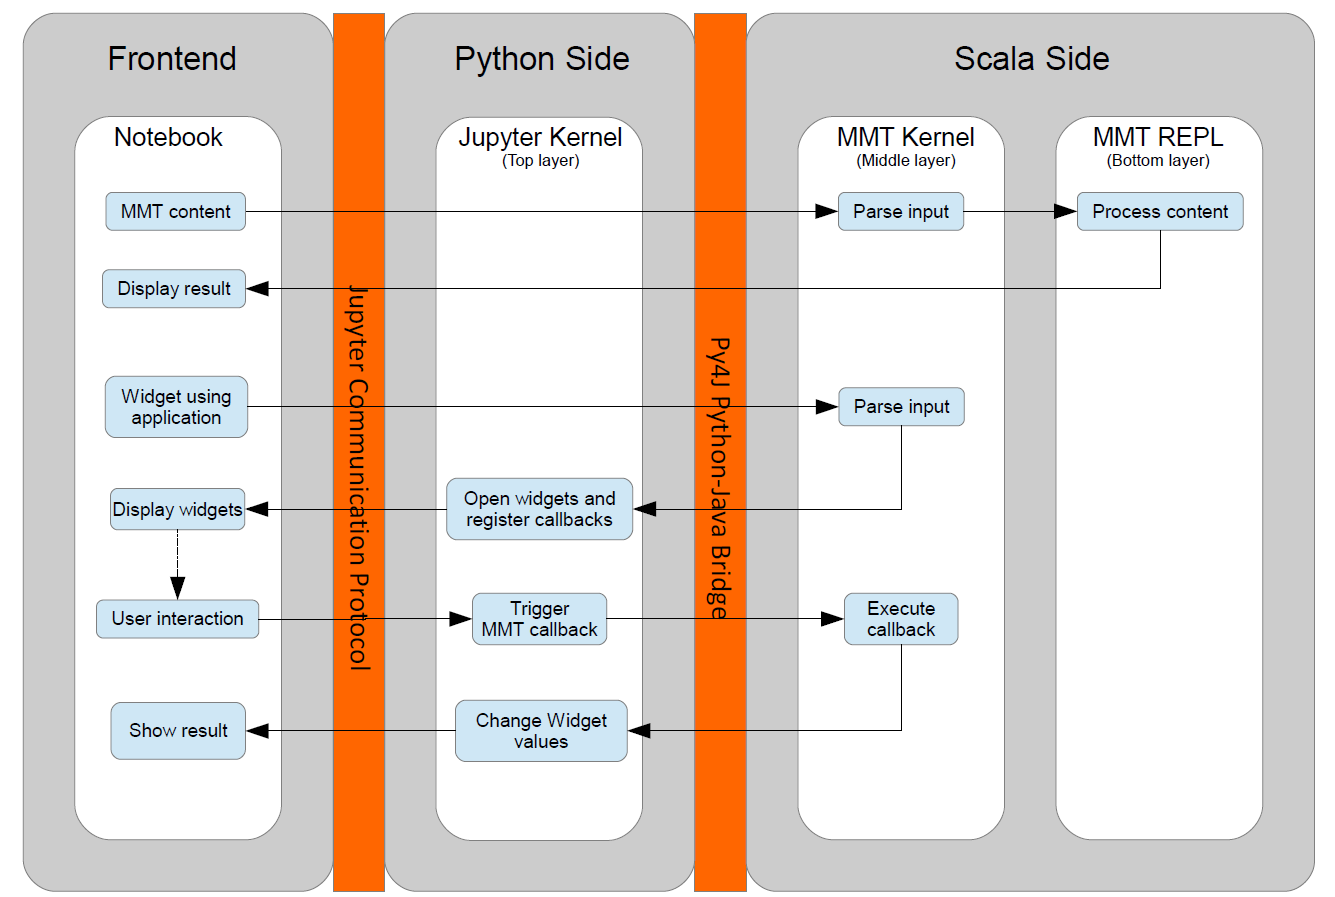
\includegraphics[width=12cm]{ArchitectureDiagram}
  \caption{Architecture diagram}\label{fig:architecture-diagram}
\end{figure}

Figure~\ref{fig:architecture-diagram} shows the details of the communication.
The upper part shows the simplest (widget-less) case: MMT content is entered in the frontend and forwarded to the bottom layer, and the response is forwarded in the opposite direction. (Steps that simply forward data from one layer to the next are not shown explicitly.)

The lower part shows a more complex widget-based interaction.
First of all, we add special management commands that are not passed on to the GUI-agnostic bottom layer.
Instead, they are identified by the middle layer, which responds by delegating to a GUI application.
This application then builds its graphical interface by calling the callbacks passed along by the top layer.
This results in a widget object in Python that is returned to the top layer and then forwarded to the frontend.

As usual, GUI components may themselves carry callback functions for handling events that are triggered by user interaction with the GUI in the frontend.
While conceptually straightforward, this leads to an unusually deep nesting of cross-programming language callbacks.
When creating a widget, the Scala-based GUI application may pass Scala callbacks $D$ whose implementation makes use of the $C$-callbacks provided by the top layer.
Thus, a user interaction triggers an MMT callback $D$ in the Python top layer, which is executed on the Scala side via Py4J, which in turn may call the Python callbacks $C$ exposed via Py4J.

%\paragraph{Jupyter/MMT Widgets}
%The use of a Python-JVM bridge pays off in particular when it allows us to reuse the widget library that is already part of the Python codebase of Jupyter.
%It allows the top layer to call the middle layer in a way that passes the Python-based kernel environment of the top layer.
%That way, the Scala-based middle layer can perform callbacks to the widget library.
%Thus, the middle layer can choose to present some of the messages returned by the bottom layer as interactive HTML using widgets.
%
%For example, when presenting a parametric theory as HTML+MathM, we can add a text input field next to every parameter.
%Whenever the strings in these fields change, the frontend notifies the top layer, which passes on the change to the middle layer.
%The middle layer then parses these strings and substitutes them in the body of the resulting declaration.
%This is similar to but more general than the typical Jupyter functionality of rerunning a notebook when an input cell changes: while Jupyter uses a list of input cells and any change affects all subsequent cells, our widget amounts to a tree structure in which input fields have local, nested scope.
%
%\ednote{@Kai: this is a simple application that we might not finish by the deliverable deadline but that you should implement nonetheless. Stay in touch with me on the details. KA: for this we would probably need a custom widget}

\paragraph*{Example: In-Document Computation}
We present a simple example of a GUI application for in-document computation as specified D4.9~\cite{ODK-D4.9}.
It is triggered by the special command \texttt{active computation} and builds a GUI consisting of a few standard Jupyter widgets: a label, a button (labeled \textit{compute}), three text input fields, and one button widget.
A concrete example can be seen in Figure~\ref{fig:ac}.
This shows a notebook in which our application is returned as the response to cell \texttt{In[1]}.


\begin{figure}[ht]\centering
  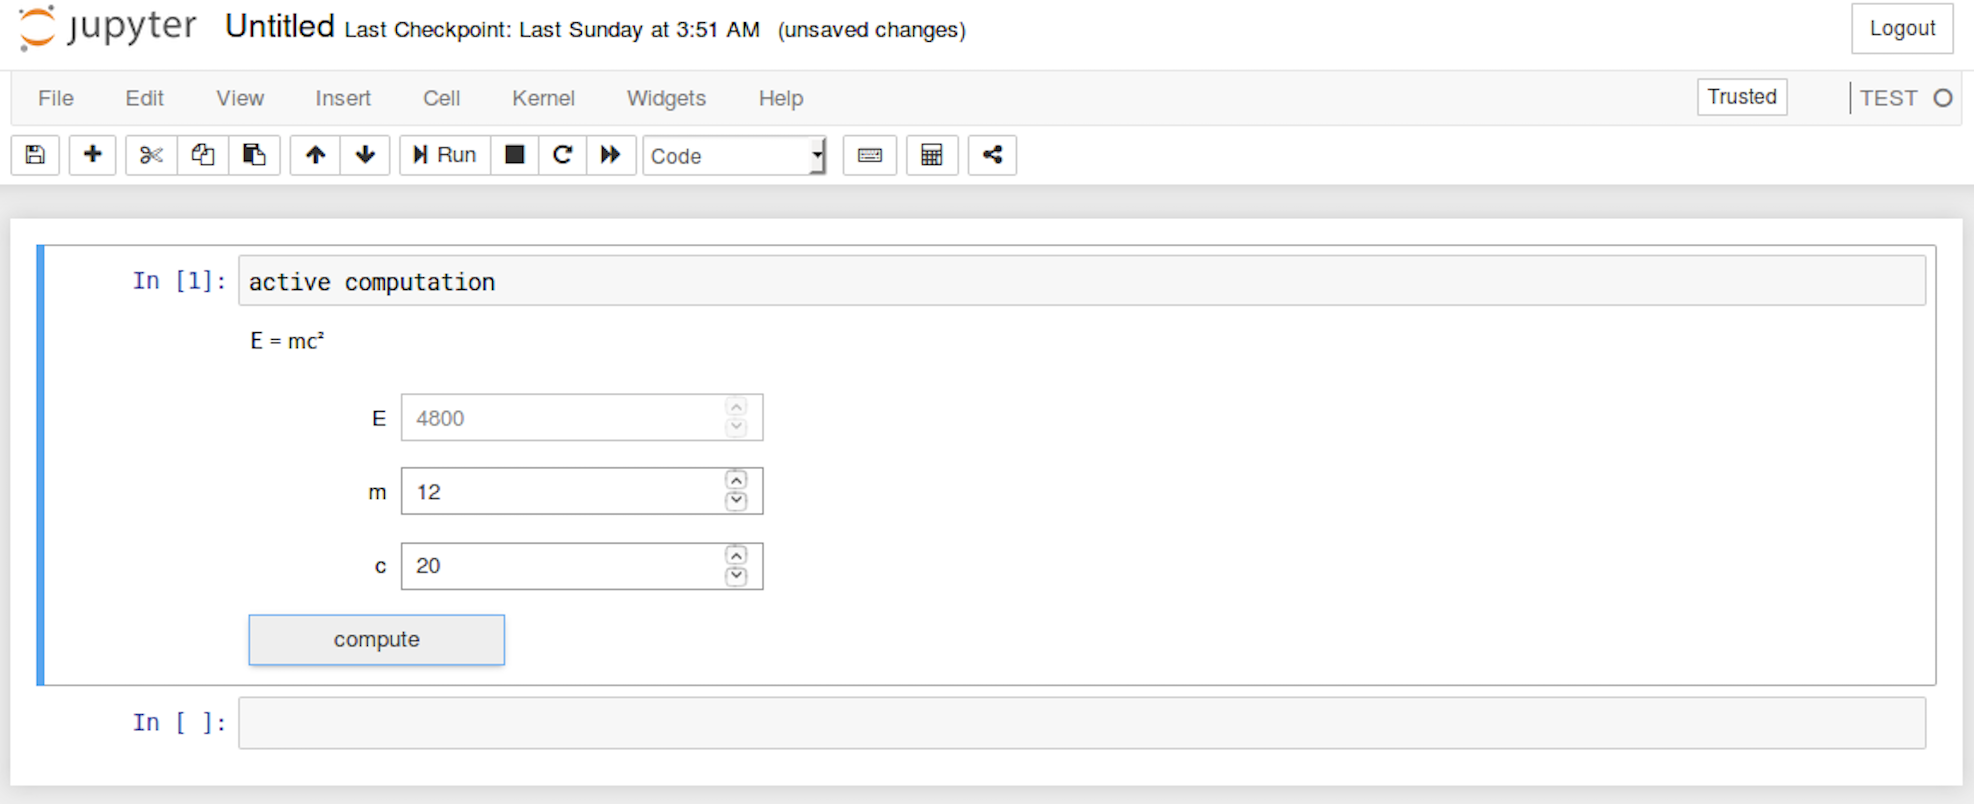
\includegraphics[width=12cm]{activecomp}
  \caption{Active Computation in Jupyter Notebooks via Jupyter/MMT Widgets}\label{fig:ac}
\end{figure}

The three text input fields contain values linked by an equation, in this case $E=mc^2$.
The user can edit these fields and press the button to compute the other values.
In that case, a the button carries the callback $D$, which results in a call to our application on the Scala side.
It uses MMT to perform the computation and then calls the $C$ callbacks to update the values in the widgets.
No additional work is needed to implement the synchronization between the Python top layer and the HTML frontend as this is a standard feature of Jupyter widgets.
\bigskip

\subsection{Document/Notebook Integration}

Our design makes it very easy to build and deploy such simple GUI applications for MMT --- we still have the full power of Jupyter widgets at our fingertips.
To achieve full document/notebook integration, as envisioned in D4.2~\cite{ODK-D4.2}, we only have to embed this notebook interface into the HTML5 presentation of the outer document (the one that contains the equation $E=mc^2$) and feed the document context information into the interior notebook as described in~\cite{ODK-D4.9} (this part of the integration can be re-used directly).

For this integration we have developed a tool that interactively generates Jupyter notebooks from HTML documents.
Figure~\ref{fig:conversionHTML} shows an example of a scientific HTML document, in which the user can use a context menu to trigger the notebook generation on a particular formula.
The context menu is generated using Javascript that picks up on annotations of MMT formulas with specific CSS classes.
Currently the author has to manually annotate the formulas, but we are working on a mechanism to automatically create it from the document context.

Figure~\ref{fig:conversionNotebook} shows the notebook created by our tool.
The downloaded notebooks can easily be uploaded to the Jupyter server on MathHub.info (see Section~\ref{sec:nb-mh}) or to a locally deployed version of the system per drag-and-drop.
Note that the generated notebook starts with several \texttt{include} declarations that import the context of the formula.

%The two predominant cell types in Jupyter notebooks are \texttt{code} and \texttt{markdown} cells. 
%Code Cells contain user input, like described in section \ref{sec:kernel:syntax}.
%The HTML elements that contain the input for these code cells are usually not visible, since they do not fit into the context of a scientific document and may not be understood by reviewers that are not familiar with MMT syntax. 
%The other cell type: markdown cells, can contain any type of plain text and support GitHub flavoured markdown. 
%Therefore markdown cells are used for providing notebooks with additional selectable information from the original HTML document.
\ednote{MK@KA/FR: For the evaluation (and Kai's thesis) we should make an sTeX document that contains $E=mc^2$ (e.g. by copying parts of \texttt{https://en.wikipedia.org/wiki/Mass-energy\_equivalence}) and really implement the in-document computation example. This would make a wonderful demo in Brussels.}

\begin{figure}[ht]\centering
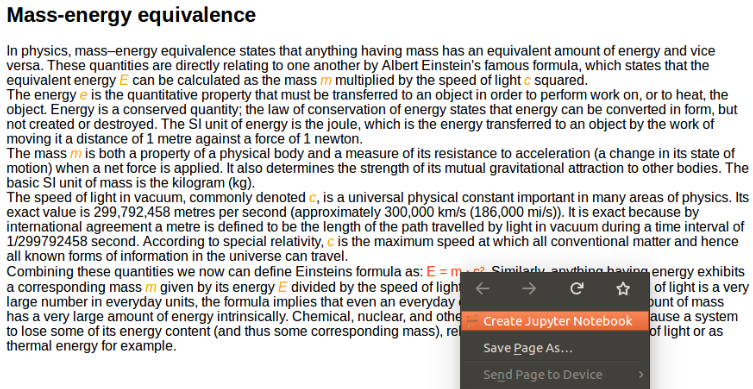
\includegraphics[width=12cm]{conversionHTML}
\caption{HTML document and the context menu for converting}
\label{fig:conversionHTML}
\end{figure}

\begin{figure}[ht]\centering
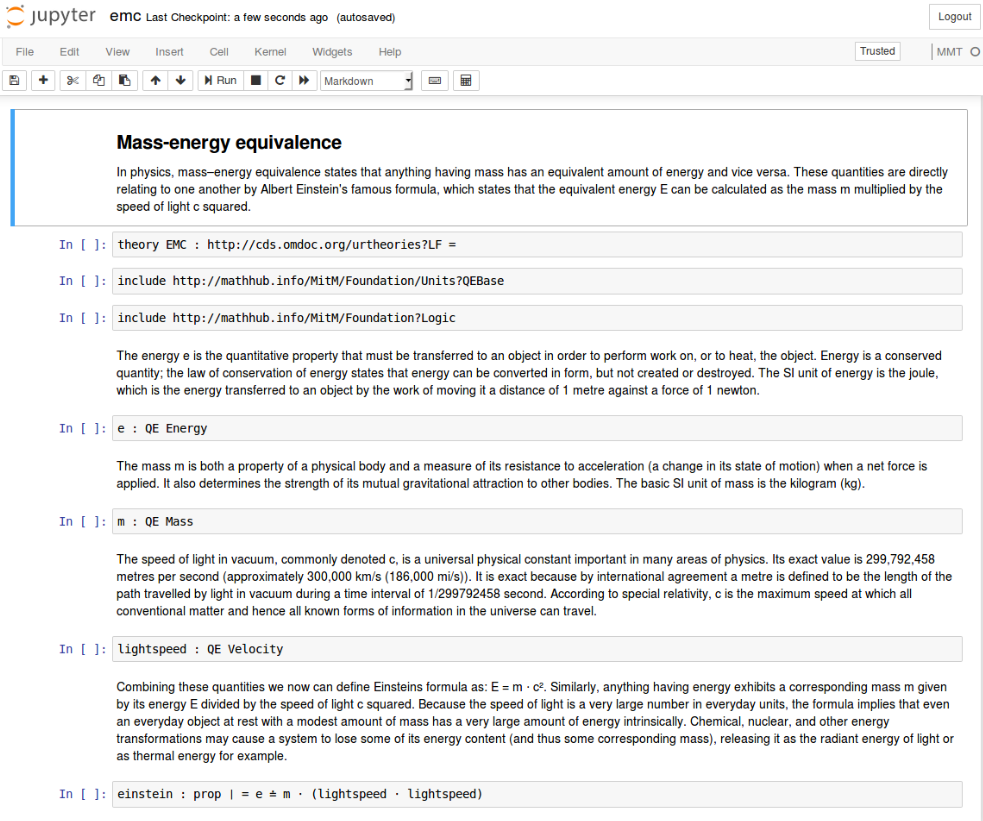
\includegraphics[width=12cm]{conversionNotebook}
\caption{The resulting Jupyter notebook}
\label{fig:conversionNotebook}
\end{figure}

%%% Local Variables:
%%% mode: latex
%%% mode: visual-line
%%% fill-column: 5000
%%% TeX-master: "report"
%%% End:

%  LocalWords:  Jupyter newpart textbf ednote centering texttt includegraphics synchronized customizable inparaenum Realizing subsubsection
